\chapter{Modelo Híbrido TCROC-Markov con Estimación NNLS}
\label{cap:tcroc_hibrido_integrado}

En este capítulo se presenta una metodología unificada que integra la discretización de regímenes económicos mediante la técnica TCROC-Markov con la estimación robusta de matrices de transición a través de Mínimos Cuadrados No Negativos (NNLS). Esta aproximación híbrida surge para superar limitaciones frecuentes en la modelización de dinámicas económicas, tales como la falta de interpretabilidad en modelos continuos y la dificultad para asegurar que las matrices de transición estimadas sean válidas desde el punto de vista estocástico.

El enfoque se compone de dos contribuciones principales:

\begin{enumerate}[label=\roman*]
    \item Una discretización precisa y estructurada que transforma series temporales continuas en estados económicos discretos y fácilmente interpretables, facilitando el análisis cualitativo y cuantitativo de regímenes económicos.
    \item Un esquema de estimación basado en NNLS que garantiza, por construcción matemática, que las matrices de transición obtenidas sean estocásticas, es decir, con entradas no negativas y columnas que suman uno, respetando las propiedades fundamentales de un proceso de Markov.
\end{enumerate}

El capítulo detalla un flujo de trabajo completo, desde la obtención de la serie temporal original y su discretización mediante la tasa de cambio relativa óptima, hasta la estimación y validación de la matriz de transición, y la posterior interpretación de la dinámica de regímenes. Se incluyen ejemplos numéricos basados en datos económicos reales, como la dinámica del Producto Interno Bruto (PIB) y la evolución de precios de combustibles, que permiten validar y ejemplificar la eficacia y aplicabilidad de la metodología propuesta.

La figura~\ref{fig:diagrama_conceptual} ilustra esquemáticamente el proceso completo, destacando cada etapa crítica y su contribución al modelo híbrido TCROC-Markov con estimación NNLS.

\begin{figure}[H]
\centering
\begin{tikzpicture}[
    node distance=2.5cm,
    process/.style={rectangle, rounded corners, minimum width=3cm, minimum height=1.6cm, text centered, text width=5cm, draw=nordGray, fill=nordSnow, text=nordDark},
    arrow/.style={thick, ->, >=stealth, nordGray}
]

\node(input) [process] {Serie Temporal Original $v(t)$};
\node(tcroc) [process, right of=input, xshift=3cm] {Cálculo de Tasa Relativa $\alpha_t$ (TCROC)};
\node(discretize) [process, below of=tcroc] {Discretización en Estados $S_t = \pi(\alpha_t)$};
\node(onehot) [process, left of=discretize, xshift=-3cm] {Codificación One-Hot y Construcción de $X_0, X_1$};
\node(nnls) [process, below of=onehot] {Estimación de $\hat{P}$ con NNLS};
\node(analysis) [process, right of=nnls, xshift=3cm] {Análisis de la Matriz y Grafo de Transición};

\draw [arrow] (input) -- (tcroc);
\draw [arrow] (tcroc) -- (discretize);
\draw [arrow] (discretize) -- (onehot);
\draw [arrow] (onehot) -- (nnls);
\draw [arrow] (nnls) -- (analysis);

\end{tikzpicture}
\caption{Diagrama conceptual de la metodología híbrida TCROC-Markov con estimación NNLS.}
\label{fig:diagrama_conceptual}
\end{figure}

% -------------------------------------------------------------------
\section[Discretización de Regímenes con TCROC-Markov]{Discretización de Regímenes Económicos\\ con TCROC-Markov}
\label{sec:discretizacion_tcroc_markov}

\subsection{Cálculo de la Tasa Relativa}
El punto de partida es la transformación de una serie temporal económica $\{v(t)\}_{t=0}^T$ en una secuencia de tasas de cambio relativas \(\alpha_t\). Para cada instante \(t\), la tasa se calcula como:
\begin{equation}
\alpha_{t,\lambda,W} = -1 + \frac{\sum_{\tau=t-W+1}^t \lambda^{t-\tau} v(\tau)v(\tau-1)}{\sum_{\tau=t-W+1}^t \lambda^{t-\tau} v(\tau-1)^2}
\label{eq:alpha_t_definition}
\end{equation}
Matemáticamente, el cociente en la Ecuación~\ref{eq:alpha_t_definition} puede interpretarse como una proyección ponderada del vector de la serie temporal \(v\) sobre su versión rezagada \(v-1\) dentro de una ventana \(W\). El factor \(\lambda\) introduce una memoria exponencial que asigna mayor importancia a las observaciones más recientes.

\subsection{Asignación de Estados}
A continuación, se define una función de cuantización \(\pi\) que mapea cada tasa continua \(\alpha_t\) a un estado discreto \(S_t\) perteneciente a un conjunto finito de regímenes económicos \(S = \{s_1, s_2, \dots, s_N\}\). Por ejemplo:

\begin{equation}
S_t = \pi(\alpha_{t,\lambda,W}) = 
\begin{cases}
s_1 & \text{si } \alpha > 0.05 \text{ (Crecimiento fuerte)} \\
s_2 & \text{si } 0 < \alpha \leq 0.05 \text{ (Crecimiento moderado)} \\
s_3 & \text{si } -0.05 \leq \alpha \leq 0 \text{ (Decrecimiento leve)} \\
s_4 & \text{si } \alpha < -0.05 \text{ (Decrecimiento severo)}
\end{cases}
\label{eq:state_assignment_pi}
\end{equation}

Este proceso genera una secuencia de estados \(\{S_t\}_{t=0}^T\), que forma la base para el modelado de transiciones.

% --- FIGURA 1: Proceso de Discretización (Versión Final) ---
\begin{figure}[H]
\centering
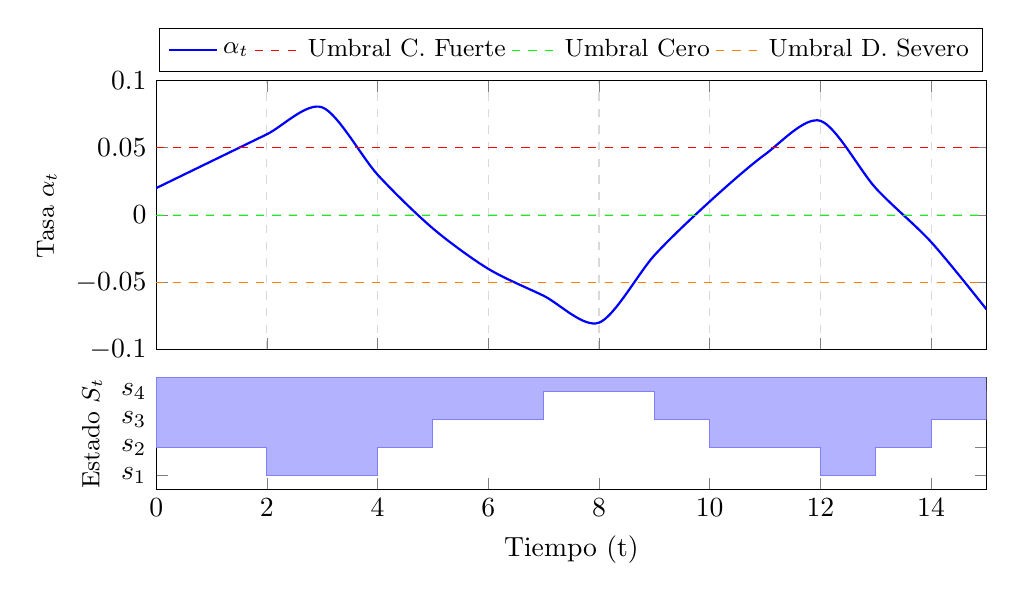
\begin{tikzpicture}
% Definición de los umbrales
\def\umbralSuperior{0.05}
\def\umbralInferior{-0.05}

\begin{axis}[
    name=plot1,
    width=\textwidth,
    height=5cm,
    xticklabels={},
    ylabel={Tasa \(\alpha_t\)},
    ylabel style={font=\small},
    grid=major,
    grid style={dashed, gray!30},
    ymin=-0.1, ymax=0.1,
    % --- AJUSTES PARA EL EJE Y ---
    ytick={-0.1, -0.05, 0, 0.05, 0.1},
    tick label style={/pgf/number format/fixed},
    % ---------------------------------
    legend style={at={(0.5,1.03)}, anchor=south, legend columns=-1, font=\small},
    xmin=0, xmax=15
]
    % Gráfico de la tasa alpha_t
    \addplot[blue, thick, smooth] coordinates {
        (0, 0.02) (1, 0.04) (2, 0.06) (3, 0.08) (4, 0.03) (5, -0.01)
        (6, -0.04) (7, -0.06) (8, -0.08) (9, -0.03) (10, 0.01) (11, 0.045)
        (12, 0.07) (13, 0.02) (14, -0.02) (15, -0.07)
    };
    \addlegendentry{\(\alpha_t\)}
    % Líneas de umbral
    \addplot[red, dashed, very thin] coordinates {(0, \umbralSuperior) (15, \umbralSuperior)};
    \addlegendentry{Umbral C. Fuerte}
    \addplot[green, dashed, very thin] coordinates {(0, 0) (15, 0)};
    \addlegendentry{Umbral Cero}
    \addplot[orange, dashed, very thin] coordinates {(0, \umbralInferior) (15, \umbralInferior)};
    \addlegendentry{Umbral D. Severo}
\end{axis}

\begin{axis}[
    name=plot2,
    at=(plot1.below south),
    anchor=above north,
    width=\textwidth,
    height=3.0cm,
    xlabel={Tiempo (t)},
    ylabel={Estado \(S_t\)},
    ylabel style={font=\small},
    ytick={1,2,3,4},
    yticklabels={$s_4$, $s_3$, $s_2$, $s_1$},
    ymin=0.5, ymax=4.5,
    xmin=0, xmax=15,
    y dir=reverse
]
    % Gráfico de escalones para estados discretos (const plot)
    \addplot[blue!50, fill=blue!30, const plot, no markers] coordinates {
        (0, 3) (1, 3) (2, 4) (3, 4) (4, 3) (5, 2) (6, 2) (7, 1)
        (8, 1) (9, 2) (10, 3) (11, 3) (12, 4) (13, 3) (14, 2) (15, 1) (16,1)
    } \closedcycle;
\end{axis}

\end{tikzpicture}
\caption{Ilustración del proceso de discretización. El panel superior muestra la evolución de la tasa continua~$\alpha_t$. El panel inferior muestra la secuencia de estados discretos~$S_t$ resultante de aplicar la función de cuantización~$\pi$.}
\label{fig:proceso_discretizacion}
\end{figure}


\begin{examplex}[Discretización y Preparación de Datos]
\label{ex:discretizacion_inflacion}

Considérese una serie temporal hipotética de inflación trimestral \(v(t)\) y los parámetros \(\lambda=1, W=2\). La secuencia de datos es:
\[ v = \{v_0, v_1, v_2, v_3, v_4\} = \{4.0, 4.1, 4.15, 4.10, 4.05 \} \]
Dado que \(W=2\), la primera tasa \(\alpha_t\) que podemos calcular es para \(t=2\).

\textbf{Cálculo para t=2:}
\begin{align*}
    \alpha_{2} &= -1 + \frac{v(2)v(1) + v(1)v(0)}{v(1)^2 + v(0)^2} \\
    &= -1 + \frac{(4.15)(4.1) + (4.1)(4.0)}{(4.1)^2 + (4.0)^2} = -1 + \frac{33.415}{32.81} \approx 0.0184
\end{align*}
Como \(0 < 0.0184 \leq 0.05\), el estado es \(\mathbf{S_2 = s_2}\).

\textbf{Cálculo para t=3:}
\begin{align*}
    \alpha_{3} &= -1 + \frac{v(3)v(2) + v(2)v(1)}{v(2)^2 + v(1)^2} \\
    &= -1 + \frac{(4.10)(4.15) + (4.15)(4.1)}{(4.15)^2 + (4.1)^2} = -1 + \frac{34.03}{34.0325} \approx -0.0001
\end{align*}
Como \(-0.05 \leq -0.0001 \leq 0\), el estado es \(\mathbf{S_3 = s_3}\).

\textbf{Cálculo para t=4:}
\begin{align*}
    \alpha_{4} &= -1 + \frac{v(4)v(3) + v(3)v(2)}{v(3)^2 + v(2)^2} \\
    &= -1 + \frac{(4.05)(4.10) + (4.10)(4.15)}{(4.10)^2 + (4.15)^2} \approx -0.0121
\end{align*}
Como \(-0.05 \leq -0.0121 \leq 0\), el estado es \(\mathbf{S_4 = s_3}\).

La secuencia de regímenes generada es \(\{S_2, S_3, S_4\} = \{s_2, s_3, s_3\}\). Esta secuencia es la que se convierte a su representación \textit{one-hot} (e.g., \(s_2 \rightarrow [0, 1, 0, 0]^T\)) para construir las matrices de datos \(X_0\) y \(X_1\), que son los insumos para la estimación descrita en la Sección \ref{sec:estimacion_nnls}.
\end{examplex}

% --- FIGURA: Visualización del Ejemplo Numérico de Discretización ---
\begin{figure}[H]
\centering
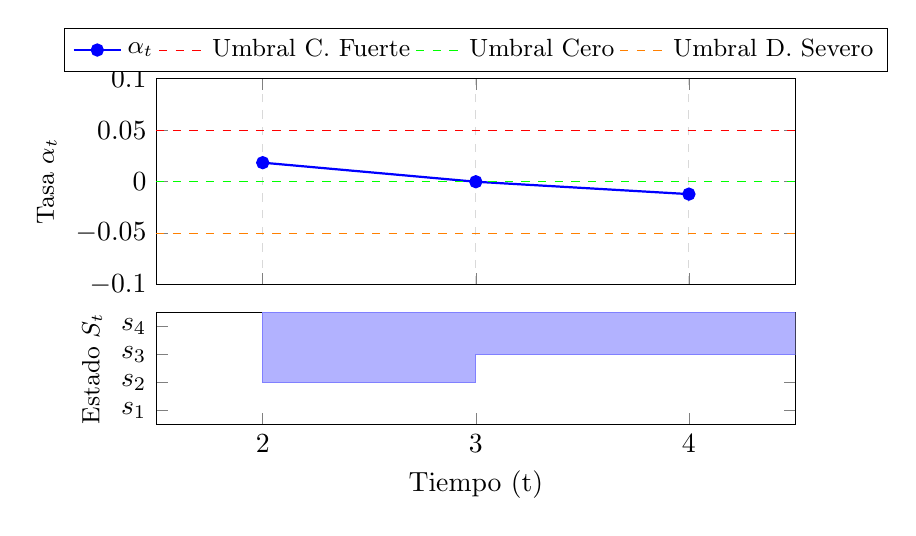
\begin{tikzpicture}
% Definición de los umbrales
\def\umbralSuperior{0.05}
\def\umbralInferior{-0.05}
\begin{axis}[
    name=plot1,
    width=0.8\textwidth,
    height=4.2cm,
    xticklabels={},
    ylabel={Tasa \(\alpha_t\)},
    ylabel style={font=\small},
    grid=major,
    grid style={dashed, gray!30},
    ymin=-0.1, ymax=0.1,
    ytick={-0.1, -0.05, 0, 0.05, 0.1},
    tick label style={/pgf/number format/fixed},
    legend style={at={(0.5,1.03)}, anchor=south, legend columns=-1, font=\small},
    xmin=1.5, xmax=4.5,
    xtick={2,3,4}
]
    % Gráfico de la tasa alpha_t (datos del ejemplo corregido)
    \addplot[blue, thick, mark=*] coordinates {
        (2, 0.0184)
        (3, -0.0001)
        (4, -0.0121)
    };
    \addlegendentry{\(\alpha_t\)}
    % Líneas de umbral
    \addplot[red, dashed, very thin] coordinates {(1.5, \umbralSuperior) (4.5, \umbralSuperior)};
    \addlegendentry{Umbral C. Fuerte}
    \addplot[green, dashed, very thin] coordinates {(1.5, 0) (4.5, 0)};
    \addlegendentry{Umbral Cero}
    \addplot[orange, dashed, very thin] coordinates {(1.5, \umbralInferior) (4.5, \umbralInferior)};
    \addlegendentry{Umbral D. Severo}
\end{axis}
\begin{axis}[
    name=plot2,
    at=(plot1.below south),
    anchor=above north,
    width=0.8\textwidth,
    height=3.0cm,
    xlabel={Tiempo (t)},
    ylabel={Estado \(S_t\)},
    ylabel style={font=\small},
    ytick={1,2,3,4},
    yticklabels={$s_4$, $s_3$, $s_2$, $s_1$},
    ymin=0.5, ymax=4.5,
    xmin=1.5, xmax=4.5,
    xtick={2,3,4},
    y dir=reverse
]
    % Gráfico de escalones para estados discretos (datos del ejemplo corregido)
    \addplot[blue!50, fill=blue!30, const plot, no markers] coordinates {
        (2, 3)
        (3, 2)
        (4, 2)
        (5, 2) % Punto extra para dibujar el último escalón
    } \closedcycle;
\end{axis}
\end{tikzpicture}
\caption{Visualización del proceso de discretización para el Ejemplo \ref{ex:discretizacion_inflacion}. El panel superior muestra los valores calculados de la tasa \(\alpha_t\). El panel inferior muestra la secuencia de estados discretos \(\{s_2, s_3, s_3\}\) resultante.}
\label{fig:discretizacion_ejemplo_numerico}
\end{figure}

\begin{examplex}[Discretización del PIB per cápita usando TCROC]
\label{ex:discretizacion_tcroc}
Considérese la serie temporal del PIB per cápita en Lempiras a precios constantes de Honduras (2000--2023), presentada en la Tabla~\ref{tbl:SeriesEvolution}. Aplicamos el paso de discretización TCROC con ventana \(W = 2\) y factor de memoria \(\lambda = 1\), usando la fórmula:
\[
\alpha_t = -1 + \frac{v(t)v(t-1) + v(t-1)v(t-2)}{v(t-1)^2 + v(t-2)^2}, \quad t \geq 2.
\]

\textbf{Cálculo para \(t=2\) (año 2002):}
\begin{align*}
    \alpha_{2} &= -1 + \frac{v(2)v(1) + v(1)v(0)}{v(1)^2 + v(0)^2} \\
    &= -1 + \frac{(16381.9)(16211.7) + (16211.7)(16214.3)}{(16211.7)^2 + (16214.3)^2} \\
    &= -1 + \frac{528\,440\,000}{525\,724\,053} \approx 0.0052
\end{align*}
Como \(-0.01 \leq 0.0052 \leq 0.02\), el estado es \(\mathbf{S_2 = s_2}\).

Los valores de \(\alpha_t\) para \(t = 3\) hasta \(t = 23\) se calcularon con la misma fórmula. La siguiente tabla resume los resultados y la clasificación en cuatro regímenes:

\begin{itemize}
    \item  \(s_1\): \(\alpha_t < -0.01\) (contracción fuerte)
    \item  \(s_2\): \(-0.01 \leq \alpha_t \leq 0.02\) (estabilidad o crecimiento débil)
    \item  \(s_3\): \(0.02 < \alpha_t \leq 0.04\) (crecimiento moderado)
    \item  \(s_4\): \(\alpha_t > 0.04\) (crecimiento fuerte)
\end{itemize}

\begin{center}
\begin{tabular}{c|c|c|c}
\(t\) & Año & \(\alpha_t\) & Estado \\
\hline
2  & 2002 & 0.0052 & \(s_2\) \\
3  & 2003 & 0.0147 & \(s_2\) \\
4  & 2004 & 0.0277 & \(s_3\) \\
5  & 2005 & 0.0358 & \(s_3\) \\
6  & 2006 & 0.0381 & \(s_3\) \\
7  & 2007 & 0.0393 & \(s_3\) \\
8  & 2008 & 0.0282 & \(s_3\) \\
9  & 2009 & -0.0136 & \(s_1\) \\
10 & 2010 & -0.0167 & \(s_1\) \\
11 & 2011 & 0.0166 & \(s_2\) \\
12 & 2012 & 0.0186 & \(s_2\) \\
13 & 2013 & 0.0139 & \(s_2\) \\
14 & 2014 & 0.0095 & \(s_2\) \\
15 & 2015 & 0.0151 & \(s_2\) \\
16 & 2016 & 0.0192 & \(s_2\) \\
17 & 2017 & 0.0246 & \(s_3\) \\
18 & 2018 & 0.0241 & \(s_3\) \\
19 & 2019 & 0.0134 & \(s_2\) \\
20 & 2020 & -0.0500 & \(s_1\) \\
21 & 2021 & -0.0106 & \(s_1\) \\
22 & 2022 & 0.0611 & \(s_4\) \\
23 & 2023 & 0.0211 & \(s_3\) \\
\end{tabular}
\end{center}

La secuencia de regímenes resultante es:
\[
\{S_t\}_{t=2}^{23} = \{s_2, s_2, s_3, s_3, s_3, s_3, s_3, s_1, s_1, s_2, s_2, s_2, s_2, s_2, s_2, s_3, s_3, s_2, s_1, s_1, s_4, s_3\}
\]
Esta secuencia se codifica en formato \textit{one-hot} para construir las matrices de datos \(X_0\) y \(X_1\), utilizadas en la estimación de la matriz de transición mediante NNLS (Sección~\ref{sec:estimacion_nnls}).
\end{examplex}

% --- FIGURA: Proceso de Discretización (Completo, Datos Reales, Formato Final) ---
\begin{figure}[H]
\centering
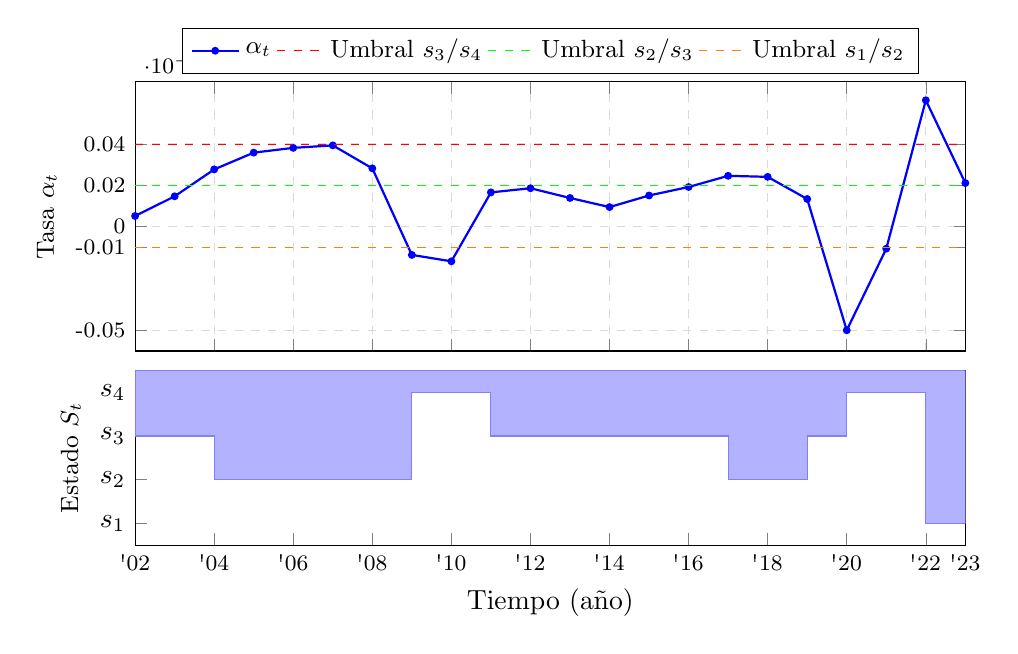
\begin{tikzpicture}

% Definición de umbrales
\def\umbralSuperior{0.04}
\def\umbralMedio{0.02}
\def\umbralInferior{-0.01}

\begin{axis}[
    name=plot1,
    width=\textwidth,
    height=5cm,
    xticklabels={},
    ylabel={Tasa \(\alpha_t\)},
    ylabel style={font=\small},
    grid=major,
    grid style={dashed, gray!30},
    ymin=-0.06, ymax=0.07,
    ytick={-0.05, -0.01, 0, 0.02, 0.04},
    yticklabels={-0.05, -0.01, 0, 0.02, 0.04},
    tick label style={font=\footnotesize, /pgf/number format/fixed},
    legend style={at={(0.5,1.03)}, anchor=south, legend columns=4, font=\small},
    xmin=0, xmax=21,
    enlarge x limits=false,
    clip mode=individual
]
    % Datos de alpha_t (t de 2 a 23) → x = t - 2
    \addplot[blue, thick, mark=*, mark size=1pt] coordinates {
        (0, 0.0052)  % '02
        (1, 0.0147)  % '03
        (2, 0.0277)  % '04
        (3, 0.0358)  % '05
        (4, 0.0381)  % '06
        (5, 0.0393)  % '07
        (6, 0.0282)  % '08
        (7, -0.0136) % '09
        (8, -0.0167) % '10
        (9, 0.0166)  % '11
        (10, 0.0186) % '12
        (11, 0.0139) % '13
        (12, 0.0095) % '14
        (13, 0.0151) % '15
        (14, 0.0192) % '16
        (15, 0.0246) % '17
        (16, 0.0241) % '18
        (17, 0.0134) % '19
        (18, -0.0500) % '20
        (19, -0.0106) % '21
        (20, 0.0611)  % '22
        (21, 0.0211)  % '23
    };
    \addlegendentry{\(\alpha_t\)}
    % Líneas de umbral
    \addplot[red, dashed, very thin] coordinates {(0, \umbralSuperior) (21, \umbralSuperior)};
    \addlegendentry{Umbral \(s_3/s_4\)}
    \addplot[green, dashed, very thin] coordinates {(0, \umbralMedio) (21, \umbralMedio)};
    \addlegendentry{Umbral \(s_2/s_3\)}
    \addplot[orange, dashed, very thin] coordinates {(0, \umbralInferior) (21, \umbralInferior)};
    \addlegendentry{Umbral \(s_1/s_2\)}
\end{axis}

\begin{axis}[
    name=plot2,
    at=(plot1.below south),
    anchor=above north,
    width=\textwidth,
    height=3.8cm,
    xlabel={Tiempo (año)},
    xtick={0,2,4,6,8,10,12,14,16,18,20,21},
    xticklabel style={font=\footnotesize},
    xticklabels={\textquotesingle02,\textquotesingle04,\textquotesingle06,\textquotesingle08,\textquotesingle10,\textquotesingle12,\textquotesingle14,\textquotesingle16,\textquotesingle18,\textquotesingle20,\textquotesingle22,\textquotesingle23},
    ylabel={Estado \(S_t\)},
    ylabel style={font=\small},
    ytick={1,2,3,4},
    yticklabels={$s_4$, $s_3$, $s_2$, $s_1$},
    ymin=0.5, ymax=4.5,
    xmin=0, xmax=21,
    y dir=reverse,
    enlarge x limits=false,
    tick align=inside
]
    % Secuencia de estados
    \addplot[blue!50, fill=blue!30, const plot, no markers] coordinates {
        (0, 2)  % '02: s2
        (1, 2)  % '03: s2
        (2, 3)  % '04: s3
        (3, 3)  % '05: s3
        (4, 3)  % '06: s3
        (5, 3)  % '07: s3
        (6, 3)  % '08: s3
        (7, 1)  % '09: s1
        (8, 1)  % '10: s1
        (9, 2)  % '11: s2
        (10, 2) % '12: s2
        (11, 2) % '13: s2
        (12, 2) % '14: s2
        (13, 2) % '15: s2
        (14, 2) % '16: s2
        (15, 3) % '17: s3
        (16, 3) % '18: s3
        (17, 2) % '19: s2
        (18, 1) % '20: s1
        (19, 1) % '21: s1
        (20, 4) % '22: s4
        (21, 3) % '23: s3
    } \closedcycle;
\end{axis}

\end{tikzpicture}
\caption{Proceso completo de discretización del PIB per cápita en Lempiras (2002--2023). El panel superior muestra la evolución de la tasa~$\alpha_t$; el inferior, la secuencia de estados discretos~$S_t$. Se observan regímenes de contracción (2009, 2020), estabilidad y crecimiento fuerte~(2022).}
\label{fig:discretizacion_completa_real}  % Label actualizado
\end{figure}

La dinámica de los regímenes económicos para el PIB per cápita, visible en la Figura~\ref{fig:discretizacion_completa_real}, ofrece una perspectiva cuantitativa de la historia económica reciente de Honduras. Se pueden extraer dos conclusiones principales:

\paragraph{Persistencia de Regímenes Durante un Período Político Extendido}
Se observa una notable persistencia de los estados \(s_2\) (estabilidad) y \(s_3\) (crecimiento moderado) durante la mayor parte del período analizado, particularmente entre 2004-2008 y 2011-2019. Este comportamiento de estabilidad y crecimiento predecible coincide en gran medida con los períodos de gobierno del Partido Nacional, incluyendo la administración de Juan Orlando Hernández (2014-2022). Las transiciones abruptas a \(s_1\) (contracción) en 2009 y 2020 marcan eventos de crisis bien conocidos (la crisis política de 2009 y la pandemia de COVID-19), interrumpiendo estos largos ciclos de estabilidad.

\paragraph{El Estado \(s_4\) como Anomalía Post-Pandemia}
La aparición única del estado \(s_4\) (crecimiento fuerte) en el año 2022 es particularmente significativa. Este régimen, que no se observa en ningún otro punto de los 22 años analizados, puede interpretarse como un efecto de "rebote" o una corrección anómala de la economía tras la drástica contracción de 2020. Su carácter excepcional sugiere que no representa una dinámica estructural sostenible, sino más bien una consecuencia transitoria de la recuperación post-COVID y de las condiciones macroeconómicas globales de ese año. La escasez de este estado en la muestra limita la capacidad del modelo para predecir eventos de crecimiento tan acelerado.

\subsection{Análisis de Sensibilidad de los Parámetros de Discretización}
La discretización de la serie temporal mediante TCROC depende de dos hiperparámetros clave: la ventana de tiempo $W$ y el factor de memoria $\lambda$. Para evaluar la robustez de nuestra discretización, se realizó un análisis de sensibilidad exhaustivo sobre los datos del PIB per cápita, variando $W \in \{2, 3, 4, 5\}$ y $\lambda$ en el rango $[0.80, 1.0]$. La Tabla~\ref{tab:sensibilidad_tcroc} presenta una selección representativa de estos resultados. El código completo utilizado para generar estos datos se encuentra en el Apéndice~\ref{apx:codigo_sensibilidad}.

\begin{table}[H]
\centering
\caption{Análisis de sensibilidad: Distribución de estados (\%) del PIB per cápita según los parámetros $W$ y $\lambda$.}
\label{tab:sensibilidad_tcroc}
\begin{tabular}{cc|cccc}
\hline
\textbf{$W$} & \textbf{$\lambda$} & \textbf{\% $s_1$} & \textbf{\% $s_2$} & \textbf{\% $s_3$} & \textbf{\% $s_4$} \\
\hline
\textbf{2} & \textbf{1.00} & \textbf{18.2} & \textbf{40.9} & \textbf{36.4} & \textbf{4.5} \\
2 & 0.90 & 13.6 & 45.5 & 36.4 & 4.5 \\
\hline
3 & 1.00 & 4.8 & 57.1 & 33.3 & 4.8 \\
3 & 0.80 & 4.8 & 57.1 & 38.1 & 0.0 \\
\hline
4 & 1.00 & 5.0 & 70.0 & 25.0 & 0.0 \\
4 & 0.80 & 5.0 & 65.0 & 30.0 & 0.0 \\
\hline
5 & 1.00 & 0.0 & 79.0 & 21.1 & 0.0 \\
5 & 0.80 & 5.3 & 68.4 & 26.3 & 0.0 \\
\hline
\end{tabular}
\end{table}

Del análisis se desprenden dos conclusiones clave. Primero, \textbf{la metodología es altamente robusta a la elección de $\lambda$}; para una ventana $W$ fija, las variaciones en el factor de memoria tienen un impacto mínimo en la distribución de estados. Esto justifica la elección de $\lambda=1.0$ por su simplicidad y efectividad.\\

Segundo, \textbf{el parámetro más influyente es la ventana $W$}, que actúa como un operador de suavizado. A medida que $W$ aumenta, la detección de regímenes extremos ($s_1$ y $s_4$) disminuye, favoreciendo al estado de estabilidad ($s_2$). Se seleccionó $W=2$ para el estudio principal, ya que representa un equilibrio que, si bien confirma el predominio de la estabilidad, es lo suficientemente sensible para capturar las contracciones económicas agudas correspondientes a eventos históricos conocidos. La consistencia de los resultados a través de los parámetros valida la fiabilidad de las conclusiones del modelo.\\



Adicionalmente, la elección de una ventana corta como $W=2$ se alinea conceptualmente con la propiedad de Markov de primer orden que se asume en la fase de modelado. Si bien la propiedad de Markov se aplica a la secuencia de estados ($S_t$) y no a los datos brutos ($v(t)$), el uso de una ventana de discretización mínima evita incorporar una memoria a largo plazo en la definición de los propios estados, manteniendo así la simplicidad y consistencia metodológica en todo el proceso.

% -------------------------------------------------------------------
% SECCIÓN 3: Estimación de la Matriz de Transición Lineal con NNLS
% ------------------------------------------------------------------
\section{Estimación de la Matriz de Transición Lineal con NNLS}
\label{sec:estimacion_nnls}

% --- VERSIÓN FINAL PARA LA INTRODUCCIÓN DE LA SECCIÓN 3 ---

Una vez obtenida la secuencia de estados discretos $\{S_t\}_{t=0}^{T}$, el siguiente paso es modelar su dinámica. Asumiendo un proceso de Markov de primer orden, la relación se describe mediante el modelo lineal $x(t+1) = Px(t)$. Para estimar la matriz de transición $P$, se emplea un enfoque de \textbf{Mínimos Cuadrados No Negativos (NNLS)}, siguiendo la metodología detallada en Vides y Lopez Gutierrez (2025)~\cite{vides_lopez_srep_2025}.

Este método es fundamental porque garantiza, por construcción, las propiedades estocásticas de la matriz estimada ($\hat{P}_{ij} \geq 0$ y $\mathbf{1}^T \hat{P} = \mathbf{1}^T$), resolviendo el siguiente problema de optimización:
\begin{equation}
\hat{P} = \arg\min_{P \in \mathbb{R}^{N \times N}} \| X_1 - P X_0 \|_F^2 \quad \text{sujeto a} \quad P_{ij} \geq 0 \text{ y } \mathbf{1}^T P = \mathbf{1}^T.
\label{eq:nnls_optim_formal}
\end{equation}
Este enfoque robusto evita soluciones inadmisibles, como probabilidades de transición negativas, que podrían surgir con estimadores de mínimos cuadrados ordinarios no restringidos. La solución a este problema se basa en algoritmos clásicos y eficientes, como el propuesto en la obra seminal de Lawson y Hanson (1995)~\cite{LawsonHanson1995}.

% --- FIN DEL BLOQUE ---

\subsection{Formulación Matemática y Solución Constructiva}

El objetivo es identificar la matriz de transición \(\hat{P}\) que minimiza el error de predicción en un paso. Dadas las matrices de datos \(X_0\) (estados en \(t\)) y \(X_1\) (estados en \(t+1\)), el problema de optimización se plantea como la minimización de la norma de Frobenius del error residual:
\begin{equation}
\hat{P} = \arg\min_{P \in \mathbb{S}(N,N)} \| X_1 - P X_0 \|_F^2
\label{eq:nnls_frobenius}
\end{equation}

donde \(\mathbb{S}_{N,N}(\mathbb{R}) = \{P \in \mathbb{R}^{N \times N} : P_{ij} \geq 0,\, \mathbf{1}^T P = \mathbf{1}^T \}\) es el conjunto de matrices estocásticas (por columnas) de tamaño \(N \times N\).

\begin{corollary}[del Teorema 3 en \cite{BanegasVides2025}]
\label{cor:existencia_p_hat_constructivo}
El problema de estimación planteado en la Ecuación~\ref{eq:nnls_frobenius} admite una solución constructiva en el espacio de matrices estocásticas.
\end{corollary}

\begin{proof}[Prueba constructiva]


La prueba sigue los pasos algorítmicos para transformar el problema matricial en un sistema lineal resoluble. La ecuación matricial del modelo, \(X_1 = \hat{P} X_0\), se linealiza aplicando el operador de \textbf{vectorización} (\(\text{vec}(\cdot)\)), que apila las columnas de una matriz en un único vector columna (i.e., \(\text{vec}(A)=[A_{11}, A_{21}, \dots, A_{nn}]^T\)). Utilizando la identidad del producto de Kronecker \(\text{vec}(ABC) = (C^T \otimes A)\text{vec}(B)\), se obtiene:

\begin{equation}
\text{vec}(X_1) = (X_0^T \otimes I_N) \text{vec}(\hat{P})
\end{equation}
Este es un sistema lineal de la forma \(b = \mathcal{A}c\), donde \(c = \text{vec}(\hat{P})\) es el vector de incógnitas, \(\mathcal{A} = X_0^T \otimes I_N\) es la matriz de diseño, y \(b = \text{vec}(X_1)\) es el vector de observaciones. El problema de minimización se convierte en \(\min_{c} \|\mathcal{A}c - b\|_2^2\), sujeto a las restricciones que definen una matriz estocástica.

Las restricciones se traducen al dominio vectorial:
\begin{itemize}
    \item La \textbf{no negatividad} (\(\hat{P}_{ij} \geq 0\)) es equivalente a la restricción de desigualdad \(c \ge 0\).
    \item La \textbf{suma de columnas unitaria} (\(\sum_{i=1}^N \hat{P}_{ij} = 1\)) se formula como un sistema de restricciones de igualdad lineal \(\mathcal{C}c = \mathbf{1}_N\), con \(\mathcal{C} = I_N \otimes \mathbf{1}_N^T\).
\end{itemize}
Ambas condiciones se integran en un único problema de Mínimos Cuadrados No Negativos (NNLS) a través de un sistema aumentado, cuya solución \(\hat{c}\) se encuentra al resolver:
\begin{equation}
\hat{c} = \arg\min_{c \geq 0} \left\| \begin{bmatrix} \mathcal{A} \\ w\mathcal{C} \end{bmatrix} c - \begin{bmatrix} b \\ w\mathbf{1}_N \end{bmatrix} \right\|_2^2
\label{eq:nnls_final_problem}
\end{equation}
Dado que el funcional objetivo es cuadrático y el conjunto de factibilidad es convexo y no vacío, la existencia de un minimizador \(\hat{c}\) está garantizada. La solución \(\hat{P} = \text{vec}^\dagger(\hat{c})\) es, por construcción, estocástica. Este procedimiento algorítmico, implementado en la función \texttt{SRep}, demuestra constructivamente la existencia de la solución \cite{BanegasVides2025, vides_lopez_srep_2025}.
\end{proof}

\begin{remark}[Sobre la unicidad de la solución]
Dado que el funcional objetivo en la Ecuación~\ref{eq:nnls_frobenius}, la norma de Frobenius al cuadrado, es estrictamente convexo, y el conjunto factible \(\mathbb{S}_{N,N}(\mathbb{R})\) también es convexo, el problema de optimización admite un minimizador global único. Por lo tanto, la matriz de transición \(\hat{P}\) estimada mediante este procedimiento no solo existe, sino que es única.
\end{remark}

\begin{examplex}[Estimación Validada de la Matriz de Transición con NNLS]
\label{ex:estimacion_nnls_pib_completa}
A partir de la secuencia de estados discretos obtenida mediante TCROC (Ejemplo~\ref{ex:discretizacion_tcroc}), se procede a estimar la matriz de transición \(\hat{P}\) utilizando el enfoque de Mínimos Cuadrados No Negativos (NNLS). La secuencia completa de estados, para \(t = 2\) hasta \(t = 23\) (2002--2023), la secuencia \( \{S_t\}_{t=2}^{23} \)
 es:
\begin{figure}[htbp]
\centering
\begin{adjustbox}{max width=\textwidth}
\begin{tikzpicture}[
    state/.style={minimum width=1.6cm, minimum height=1.5cm, text centered, inner sep=0pt},
    label/.style={font=\Large\bfseries}
]

% Posición inicial en X
\def\xpos{0}

% Lista de estados y años con colores explícitos
% Formato: letra, color, número, año
\foreach \name/\color/\num/\year in {
    S2/blue!10/2/02,
    S2/blue!10/2/03,
    S3/green!10/3/04,
    S3/green!10/3/05,
    S3/green!10/3/06,
    S3/green!10/3/07,
    S3/green!10/3/08,
    S1/red!10/1/09,
    S1/red!10/1/10,
    S2/blue!10/2/11,
    S2/blue!10/2/12,
    S2/blue!10/2/13,
    S2/blue!10/2/14,
    S2/blue!10/2/15,
    S2/blue!10/2/16,
    S3/green!10/3/17,
    S3/green!10/3/18,
    S2/blue!10/2/19,
    S1/red!10/1/20,
    S1/red!10/1/21,
    S4/orange!20/4/22,
    S3/green!10/3/23
} {
    % Dibujar recuadro coloreado con texto S<num>
    \node[draw=black, fill=\color, state] (S\year) at (\xpos, 0) {\Large\textbf{S\num}};
    % Etiqueta del año debajo
    \node[label] at (S\year.south) [below=1mm] {\year};
    % Avanzar posición horizontal
    \pgfmathsetmacro{\xpos}{\xpos + 1.6}
    \xdef\xpos{\xpos}
}
\end{tikzpicture}
\end{adjustbox}
\caption{Secuencia temporal de estados discretos obtenidos mediante TCROC.}
\label{fig:secuencia_estados}
\end{figure}

Con \(N = 4\) estados definidos como:
\begin{itemize}
    \item \(s_1\): Contracción (\(\alpha_t < -0.01\))
    \item \(s_2\): Estabilidad (\(-0.01 \leq \alpha_t \leq 0.02\))
    \item \(s_3\): Crecimiento moderado (\(0.02 < \alpha_t \leq 0.04\))
    \item \(s_4\): Crecimiento fuerte (\(\alpha_t > 0.04\))
\end{itemize}

Representados en formato \textit{one-hot}:
\[
s_1 = \begin{bmatrix} 1 \\ 0 \\ 0 \\ 0 \end{bmatrix},\quad
s_2 = \begin{bmatrix} 0 \\ 1 \\ 0 \\ 0 \end{bmatrix},\quad
s_3 = \begin{bmatrix} 0 \\ 0 \\ 1 \\ 0 \end{bmatrix},\quad
s_4 = \begin{bmatrix} 0 \\ 0 \\ 0 \\ 1 \end{bmatrix}
\]

Se construyen las matrices de datos:
\begin{itemize}
    \item \(X_0 = [x(2), x(3), \dots, x(22)] \in \mathbb{R}^{4 \times 21}\): estados actuales.
    \item \(X_1 = [x(3), x(4), \dots, x(23)] \in \mathbb{R}^{4 \times 21}\): estados siguientes.\\
\end{itemize}

\paragraph{Construcción de las Matrices de Datos}
A partir de la secuencia de estados y su codificación \textit{one-hot}, se construyen las matrices de datos \(X_0\) y \(X_1\). La matriz \(X_0\) se forma con los vectores de los estados actuales (\(t=2\) a \(t=22\)), y la matriz \(X_1\) con los vectores de los estados siguientes (\(t=3\) a \(t=23\)).

\begin{equation*}
\resizebox{0.6\textwidth}{!}{$
X_0 =
\begin{bmatrix}
0 , 0 , 0 , 0 , 0 , 0 , 0 , 1 , 1 , 0 , 0 , 0 , 0 , 0 , 0 , 0 , 0 , 0 , 1 , 1 , 0 \\
1 , 1 , 0 , 0 , 0 , 0 , 0 , 0 , 0 , 1 , 1 , 1 , 1 , 1 , 1 , 0 , 0 , 1 , 0 , 0 , 0 \\
0 , 0 , 1 , 1 , 1 , 1 , 1 , 0 , 0 , 0 , 0 , 0 , 0 , 0 , 0 , 1 , 1 , 0 , 0 , 0 , 0 \\
0 , 0 , 0 , 0 , 0 , 0 , 0 , 0 , 0 , 0 , 0 , 0 , 0 , 0 , 0 , 0 , 0 , 0 , 0 , 0 , 1
\end{bmatrix}
$}
\label{eq:matrix_X0}
\end{equation*}

\begin{equation*}
\resizebox{0.6\textwidth}{!}{$
X_1 =
\begin{bmatrix}
0 , 0 , 0 , 0 , 0 , 0 , 1 , 1 , 0 , 0 , 0 , 0 , 0 , 0 , 0 , 0 , 0 , 1 , 1 , 0 , 0 \\
1 , 0 , 0 , 0 , 0 , 0 , 0 , 0 , 1 , 1 , 1 , 1 , 1 , 1 , 1 , 0 , 1 , 0 , 0 , 0 , 0 \\
0 , 1 , 1 , 1 , 1 , 1 , 0 , 0 , 0 , 0 , 0 , 0 , 0 , 0 , 0 , 1 , 1 , 0 , 0 , 0 , 1 \\
0 , 0 , 0 , 0 , 0 , 0 , 0 , 0 , 0 , 0 , 0 , 0 , 0 , 0 , 0 , 0 , 0 , 0 , 0 , 1 , 0 
\end{bmatrix}
$}
\label{eq:matrix_X1}
\end{equation*}

Estas dos matrices son la base para el conteo de transiciones y la posterior estimación con NNLS. Para estimar \(\hat{P}\), se cuenta el número de transiciones entre estados. Sea \(C \in \mathbb{Z}^{4 \times 4}\) la matriz de conteo, donde \(C_{ij}\) es el número de transiciones de \(s_j\) a \(s_i\). Esta matriz se puede calcular eficientemente a partir de las matrices de datos \(X_1\) y \(X_0\) mediante la siguiente operación:
\begin{equation}
    C = X_1 X_0^T
\end{equation}

Recorriendo los pares \((S_t, S_{t+1})\) de la secuencia, se obtiene:

\[
C = 
\begin{bmatrix}
2 & 1 & 1 & 0 \\
1 & 6 & 1 & 0 \\
0 & 2 & 5 & 1 \\
1 & 0 & 0 & 0 \\
\end{bmatrix}
\]

La matriz de transición se obtiene normalizando esta matriz de conteo por columnas:
\begin{equation}
    \hat{P}_{ij} = \frac{C_{ij}}{\sum_{k=1}^4 C_{kj}}, \quad \forall j
\end{equation}

\[
\hat{P}=
\begin{bmatrix}
0.5000 & 0.1111 & 0.1429 & 0.0000 \\
0.2500 & 0.6667 & 0.1429 & 0.0000 \\
0.0000 & 0.2222 & 0.7143 & 1.0000 \\
0.2500 & 0.0000 & 0.0000 & 0.0000
\end{bmatrix}
\]

Para validar empíricamente la correcta implementación del algoritmo de estimación propuesto en~\cite{vides_lopez_srep_2025}, se realiza un experimento numérico que consiste en dos fases. Primero, se utiliza la matriz  \(\hat{P}\) como "verdad fundamental" para simular una nueva secuencia de estados. Posteriormente, se aplica sobre estos datos simulados el algoritmo de Mínimos Cuadrados No Negativos (NNLS) implementado en la función \texttt{SRep}, cuya metodología se detalla en el Listado~\ref{lst:srep_implementacion}. El objetivo es verificar si el estimador recupera la matriz original.

La implementación completa del algoritmo \texttt{SRep} se
presenta en el Apéndice~\ref{apx:codigo_srep}
(Listado~\ref{lst:srep_implementacion}).

El resultado de la validación se evalúa calculando la matriz de diferencia entre la matriz estimada y la original (\(Ap -\hat{P}\)). Tal como se muestra a continuación, el resultado es una matriz donde todos los elementos son numéricamente cero, con errores del orden de \(10^{-13}\) atribuibles únicamente a la precisión de punto flotante:

\[
Ap -\hat{P} \approx
\begin{bmatrix}
 0 & 0 & 0 & 0 \\
 0 & 0 & 0 & 0 \\
 0 & 0 & 0 & 0 \\
 0 & 0 & 0 & 0
\end{bmatrix}
\]

Este resultado valida empíricamente que la función \texttt{SRep} implementa correctamente el estimador propuesto, logrando recuperar la matriz de transición original con alta precisión.

% --- FIGURA : Grafo de Transición de Estados ---
\begin{figure}[H]
\centering
\begin{tikzpicture}[
    node distance=3cm,
    every node/.style={fill=white, inner sep=2pt},
    state/.style={circle, draw, thick, minimum size=1.8cm, font=\small},
    arrow/.style={->, >=stealth, thick},
    prob/.style={font=\scriptsize, midway, fill=white, inner sep=1pt}
]

% Nodos (estados)
\node[state, fill=nordRed!15] (s1) at (0,0) {$s_1$ \textsc{\tiny (Contracción)}};
\node[state, fill=nordFrost!15] (s2) at (4,0) {$s_2$ \textsc{\tiny (Estabilidad)}};
\node[state, fill=nordGreen!15] (s3) at (4,-3) {$s_3$ \textsc{\tiny \shortstack{(Crecimiento\\moderado)}}};
\node[state, fill=nordYellow!15] (s4) at (0,-3) {$s_4$ \textsc{\tiny \shortstack{(Crecimiento\\fuerte)}}};


% Auto-transiciones (laços)
\draw[arrow, loop above, min distance=10mm, in=120, out=60] (s1) to node[prob] {50\%} (s1);
\draw[arrow, loop right, min distance=10mm, in=-30, out=30] (s2) to node[prob] {66.7\%} (s2);
\draw[arrow, loop below, min distance=10mm, in=-60, out=-120] (s3) to node[prob] {71.4\%} (s3);

% Transiciones entre estados
\draw[arrow] (s1) to[bend left=15] node[prob, above] {25\%} (s2);
\draw[arrow] (s1) to[bend left=15] node[prob, left] {25\%} (s4);

\draw[arrow] (s2) to[bend left=15] node[prob, pos=0.4, xshift=6pt, yshift=-6pt] {11.1\%} (s1);
\draw[arrow] (s2) to node[prob, pos=0.6, xshift=10pt, yshift=10pt] {22.2\%} (s3);

\draw[arrow] (s3) to[bend left=15] node[prob, pos=0.4, xshift=-6pt, yshift=8pt] {14.3\%} (s1);
\draw[arrow] (s3) to[bend left=15] node[prob, pos=0.6, xshift=-12pt, yshift=-8pt] {14.3\%} (s2);

\draw[arrow] (s4) to node[prob, above] {100\%} (s3);


\end{tikzpicture}
\caption{Grafo de transición estimado para los regímenes del PIB per cápita en Lempiras.}
\label{fig:grafo_transicion}
\end{figure}

\paragraph{Interpretación de la Matriz de Transición}

La matriz \(\hat{P}\) revela la dinámica subyacente del sistema:
\begin{itemize}
    \item \textbf{Estado \(s_1\) (Contracción):} Persiste con una probabilidad del 50\%, mientras que se recupera transitando a \(s_2\) (estabilidad) o a \(s_4\) (crecimiento fuerte) con una probabilidad del 25\% en cada caso.
    \item \textbf{Estado \(s_2\) (Estabilidad):} Es el régimen más persistente, con una probabilidad del 66.7\% de mantenerse. Su principal vía de salida es hacia \(s_3\) (crecimiento moderado), con un 22.2\%.
    \item \textbf{Estado \(s_3\) (Crecimiento moderado):} También es altamente estable, persistiendo con un 71.4\%. La probabilidad de retroceso a otros estados es baja.
    \item \textbf{Estado \(s_4\) (Crecimiento fuerte):} Actúa como un estado puramente transitorio. En la muestra observada, siempre es seguido por una transición al estado \(s_3\), lo que sugiere que los picos de crecimiento tienden a moderarse rápidamente.
\end{itemize}

\paragraph{Propiedades Teóricas del Estimador}
La matriz \(\hat{P}\), calculada a partir de las frecuencias relativas de transición, corresponde al \textbf{Estimador de Máxima Verosimilitud (MLE)} para una cadena de Markov de primer orden. Este estimador posee propiedades asintóticas bien establecidas.

\begin{theorem}[Consistencia del Estimador]
\label{thm:consistencia_p_hat}
Dada una cadena de Markov ergódica con una matriz de transición verdadera (e inobservable) $P$, el estimador de máxima verosimilitud $\hat{P}$, obtenido a partir de una secuencia de $T$ observaciones, es consistente. Esto implica que el estimador converge en probabilidad a la matriz verdadera a medida que el número de observaciones tiende a infinito:
$$
\hat{P} \xrightarrow{p} P \quad \text{cuando} \quad T \to \infty
$$
\end{theorem}
\begin{proof}
Por la ley fuerte de los grandes números para cadenas de Markov
ergódicas \cite{Norris1998}, las frecuencias relativas de
transición convergen casi seguramente:
\[
\hat{p}_{ij} = \frac{N_{ij}}{N_{i\cdot}}
\xrightarrow{\text{c.s.}} p_{ij},
\quad T \to \infty,
\]
donde $N_{ij} = \#\{t : S_t = i,\, S_{t+1} = j\}$ y
$N_{i\cdot} = \sum_j N_{ij}$.  Dado que la cadena es ergódica,
cada estado se visita infinitas veces, por lo que $N_{i\cdot}
\to \infty$ para todo $i$.  La convergencia
entrada-por-entrada implica $\|\hat{P} - P\|_{\max}
\xrightarrow{\text{c.s.}} 0$.  Este resultado fue establecido
formalmente por Anderson y Goodman~\cite{AndersonGoodman1957}.
El estimador NNLS coincide con el MLE bajo las restricciones de
no-negatividad, heredando así la consistencia.
\end{proof}

\noindent La inclusión de este resultado es fundamental, pues certifica que, con una cantidad suficiente de datos, nuestra metodología se aproxima al verdadero proceso generador de la dinámica de regímenes.

\paragraph{Simulación de la Evolución de la Cadena de Markov}
Para validar la capacidad del estimador SRep de recuperar la
matriz de transición original, se simula la evolución de una
cadena de Markov utilizando la matriz $\hat{P}$ estimada
previamente. Se define un estado inicial correspondiente a $s_1$
y se genera una secuencia de ocupaciones probabilísticas para
$T = 20$ pasos (véase Apéndice~\ref{apx:codigo_srep},
Listado~\ref{lst:simulacion_markov}).

La Figura~\ref{fig:evolucion_probabilidades_markov} muestra la evolución temporal de las probabilidades de ocupación para cada uno de los estados del sistema Markoviano, bajo la matriz de transición estimada \(\hat{P}\), a lo largo de 20 pasos de simulación.

\begin{figure}[H]
    \centering
    \includegraphics[width=0.8\textwidth]{figures/evolucion_probabilidades_markov.png}
    \caption{Evolución temporal de las probabilidades de ocupación de los estados \(s_1, s_2, s_3, s_4\) bajo la dinámica inducida por la matriz de transición estimada \(\hat{P}\).}
    \label{fig:evolucion_probabilidades_markov}
\end{figure}


\begin{itemize}
    \item \textbf{Estado \(s_1\) (contracción):} Inicia con probabilidad unitaria (\(1.0\)) y experimenta un descenso rápido durante los primeros 5 pasos. A partir del paso 6, la probabilidad se estabiliza alrededor de \(0.195\), oscilando mínimamente entre \(0.1957\) y \(0.1951\) hasta el final de la simulación.
    \item \textbf{Estado \(s_2\) (estabilidad):} Comienza en cero y crece de forma sostenida. Se estabiliza aproximadamente en el paso 10, alrededor de \(0.329\), mostrando una variación insignificante (\(<0.001\)) desde ese punto en adelante.
    \item \textbf{Estado \(s_3\) (crecimiento moderado):} Aunque inicia en cero, incrementa rápidamente y supera a los demás estados a partir del paso 2. A partir del paso 7, se mantiene en torno a \(0.427\), con oscilaciones menores a \(0.001\), confirmando su papel como estado dominante en el régimen estacionario.
    \item \textbf{Estado \(s_4\) (crecimiento fuerte):} Presenta un leve incremento inicial pero desciende pronto, estabilizándose en torno a \(0.0488\) a partir del paso 6. Su baja probabilidad persistente evidencia su carácter transitorio.
\end{itemize}

\noindent
\textbf{Estabilización global:}
En general, la cadena de Markov alcanza el equilibrio estacionario a partir de los pasos 10 a 12, cuando las probabilidades de todos los estados dejan de variar de manera significativa y convergen a valores constantes: \(s_1 \approx 0.195\), \(s_2 \approx 0.329\), \(s_3 \approx 0.427\) y \(s_4 \approx 0.049\). Este comportamiento confirma que el sistema converge rápidamente a un régimen estable, dominado por los estados de crecimiento moderado y estabilidad.\\

En conjunto, la dinámica observada en la gráfica es plenamente consistente con la teoría de cadenas de Markov: los estados de crecimiento moderado y estabilidad emergen como los destinos predominantes a largo plazo, mientras que los estados extremos (contracción y crecimiento fuerte) son rápidamente abandonados y sólo se presentan de manera transitoria. \\

Esta convergencia hacia regímenes centrales y estables refleja tanto la estructura de la matriz de transición estimada \(\hat{P}\) como la naturaleza realista de procesos económicos o financieros modelados por este tipo de sistemas. En definitiva, el comportamiento del sistema valida que la modelación mediante cadenas de Markov captura adecuadamente las dinámicas de persistencia y transición entre regímenes típicas en el análisis de series temporales económicas.

\end{examplex}
\subsection{Validación del Rendimiento Predictivo}
Para cuantificar la capacidad predictiva del modelo, se evaluó su rendimiento utilizando múltiples particiones de entrenamiento y prueba. Se entrenó la matriz de transición \(\hat{P}\) con porciones crecientes de la serie temporal (desde el 60\% hasta el 95\%) y se validó su capacidad para predecir el estado del siguiente período en los datos restantes. El código completo para este análisis de robustez se encuentra en el Apéndice~\ref{apx:codigo_validacion_completo}.

La Tabla~\ref{tab:rendimiento_predictivo_resumen} resume la precisión (accuracy) del modelo para cada partición.

\begin{table}[H]
\centering
\begin{tabularx}{\textwidth}{X c c}
\hline
\textbf{Entrenamiento/Prueba} & \textbf{Nº de Predicciones} & \textbf{Precisión (Accuracy)} \\
\hline
60\% / 40\% & 8 & 0.375 \\
70\% / 30\% & 6 & 0.167 \\
80\% / 20\% & 4 & 0.000 \\
90\% / 10\% & 2 & 0.000 \\
95\% / 5\%  & 1 & 0.000 \\
\hline
\end{tabularx}
\caption{Resumen del rendimiento predictivo según la partición de datos.}
\label{tab:rendimiento_predictivo_resumen}
\end{table}

Los resultados revelan un hallazgo crucial: la precisión predictiva es mayor cuando el conjunto de prueba es más grande y disminuye a cero a medida que este se reduce. Este comportamiento, aparentemente contraintuitivo, no indica un deterioro del modelo. Por el contrario, se explica porque los conjuntos de prueba más pequeños aíslan las transiciones más recientes y anómalas de la serie, particularmente el evento único del estado $s_4$ (crecimiento fuerte) en 2022. Al ser un evento sin precedentes en los datos de entrenamiento, el modelo es incapaz de predecirlo, lo que demuestra una limitación clásica de los modelos de Markov basados en datos históricos: son efectivos para capturar dinámicas recurrentes, pero su capacidad para predecir eventos únicos es inherentemente limitada por la escasez de datos.

\begin{examplex}[Definición y Discusión de Estados para Series de Combustibles]

\label{ex:estados_combustibles_discusion}

Para la discretización de las series de precios de combustibles, se definieron cuatro estados cuantitativos en función del parámetro \(\alpha\), que mide la tasa relativa de cambio en cada periodo. Estos estados se codifican como \(s1, s2, s3, s4\), que se interpretan respectivamente como \emph{caída}, \emph{estable}, \emph{subida} y \emph{alza fuerte}.\\

La función de asignación utilizada fue la siguiente:
\[
\text{estado} =
\begin{cases}
s1 & \text{si } \alpha < -0.01 \\
s2 & \text{si } -0.01 \leq \alpha \leq 0.02 \\
s3 & \text{si } 0.02 < \alpha \leq 0.04 \\
s4 & \text{si } \alpha > 0.04
\end{cases}
\]

Esta definición, aunque arbitraria, responde a un criterio homogéneo aplicado a todas las series con el fin de facilitar la comparación directa entre ellas. 

\bigskip
\noindent\textbf{Pros y Contras del enfoque:}

\begin{itemize}
    \item \textbf{Límites fijos para todas las series:}
    \begin{itemize}
        \item \textit{Pros:} Permite un marco común para análisis comparativos y es sencillo de explicar y mantener.
        \item \textit{Contras:} Puede no captar particularidades dinámicas específicas de cada serie; por ejemplo, una serie con baja variabilidad puede quedar demasiado concentrada en un solo estado.
    \end{itemize}
    \item \textbf{Límites dinámicos o personalizados para cada serie:}
    \begin{itemize}
        \item \textit{Pros:} Permite mayor sensibilidad a las fluctuaciones internas y mejor interpretación dentro de cada serie.
        \item \textit{Contras:} Dificulta la comparación entre series al no tener un sistema uniforme de estados.
    \end{itemize}
\end{itemize}

\bigskip
En este trabajo, se optó por mantener límites fijos para todas las series con el objetivo de facilitar análisis cualitativos y comparativos, a pesar de reconocer que en futuros estudios podrían explorarse límites dinámicos o adaptativos para mejorar la sensibilidad y precisión.

\bigskip
A continuación, se presentan las matrices de conteo \( C \), matrices de transición\( \hat{P} \), matrices estimadas \( A_p \) mediante la función \( \texttt{SRep} \), y la diferencia entre estas matrices para las cuatro series de precios de combustibles: \textbf{Super, Regular, Diesel} y \textbf{Kerosene}.

\bigskip
\noindent\textbf{Matrices de Conteo \(C\):}

\[
C_{\text{Super}} = \begin{bmatrix}
41 & 18 & 1 & 0 \\
19 & 327 & 6 & 0 \\
0 & 7 & 13 & 0 \\
0 & 0 & 0 & 0
\end{bmatrix}
\quad
C_{\text{Regular}} = \begin{bmatrix}
43 & 13 & 1 & 0 \\
14 & 334 & 6 & 0 \\
0 & 7 & 14 & 0 \\
0 & 0 & 0 & 0
\end{bmatrix}
\]

\[
C_{\text{Diesel}} = \begin{bmatrix}
62 & 19 & 1 & 0 \\
20 & 304 & 5 & 0 \\
0 & 6 & 11 & 2 \\
0 & 1 & 1 & 0
\end{bmatrix}
\quad
C_{\text{Kerosene}} = \begin{bmatrix}
81 & 23 & 0 & 0 \\
23 & 238 & 13 & 1 \\
0 & 13 & 25 & 4 \\
0 & 1 & 4 & 6
\end{bmatrix}
\]

Se observa que en las matrices de conteo para \textbf{Super} y \textbf{Regular}, tanto la cuarta fila como la cuarta columna son vectores nulos. Esto indica que el estado \(s_4\) (alza fuerte) es un estado transitorio no observado en estas series de datos; nunca se transita desde ni hacia él. Para un análisis más robusto y enfocado en la dinámica real, se puede reducir el espacio de estados de 4x4 a 3x3, considerando únicamente los estados activos (\(s_1, s_2, s_3\)). Las submatrices de conteo resultantes son:

\[
C_{\text{Super}}^{\text{reducida}} = \begin{bmatrix}
41 & 18 & 1 \\
19 & 327 & 6 \\
0 & 7 & 13
\end{bmatrix}
\quad
C_{\text{Regular}}^{\text{reducida}} = \begin{bmatrix}
43 & 13 & 1 \\
14 & 334 & 6 \\
0 & 7 & 14
\end{bmatrix}
\]

\bigskip
\noindent\textbf{Matrices de Transición ($\hat{P}$) (Normalizadas por columna, 3 decimales):}

\[
\hat{P}_{\text{Super}} = \begin{bmatrix}
0.683, 0.051, 0.050\\
0.317, 0.929, 0.300 \\
0.000, 0.020, 0.650
\end{bmatrix}
\quad
\hat{P}_{\text{Regular}} = \begin{bmatrix}
0.754, 0.037, 0.048 \\
0.246, 0.944, 0.286 \\
0.000, 0.020, 0.667
\end{bmatrix}
\]

\[
\hat{P}_{\text{Diesel}} = \begin{bmatrix}
0.756, 0.058, 0.056, 0.000 \\
0.244, 0.921, 0.278, 0.000 \\
0.000, 0.018, 0.611, 1.000 \\
0.000, 0.003, 0.056, 0.000
\end{bmatrix}
\quad
\hat{P}_{\text{Kerosene}} = \begin{bmatrix}
0.779, 0.084, 0.000, 0.000 \\
0.221, 0.865, 0.310, 0.091 \\
0.000, 0.047, 0.595, 0.364 \\
0.000, 0.004, 0.095, 0.545
\end{bmatrix}
\]

\bigskip
\noindent\textbf{Matrices \(A_p\) Estimadas con \( \texttt{SRep} \) (3 decimales):}

\[
A_{p, \text{Super}} = \begin{bmatrix}
0.683, 0.051, 0.050 \\
0.317, 0.929, 0.300 \\
0.000, 0.020, 0.650
\end{bmatrix}
\]

\[
A_{p, \text{Regular}} = \begin{bmatrix}
0.754, 0.037, 0.048 \\
0.246, 0.944, 0.286 \\
0.000, 0.020, 0.667
\end{bmatrix}
\]

\[
A_{p, \text{Diesel}} = \begin{bmatrix}
0.756, 0.058, 0.056, 0.000 \\
0.244, 0.921, 0.278, 0.000 \\
0.000, 0.018, 0.611, 1.000 \\
0.000, 0.003, 0.056, 0.000
\end{bmatrix}
\]

\[
A_{p, \text{Kerosene}} = \begin{bmatrix}
0.779, 0.084, 0.000, 0.000 \\
0.221, 0.865, 0.310, 0.091 \\
0.000, 0.047, 0.595, 0.364 \\
0.000, 0.004, 0.095, 0.545
\end{bmatrix}
\]

\bigskip
\noindent\textbf{Diferencia \(A_p - \hat{P}\) :}

\[
\Delta_{\text{Super}} = \begin{bmatrix}
0, 0, 0 \\
0, 0, 0 \\
0, 0, 0
\end{bmatrix}
\quad
\Delta_{\text{Regular}} = \begin{bmatrix}
0, 0, 0 \\
0, 0, 0 \\
0, 0, 0 
\end{bmatrix}
\]

\[
\Delta_{\text{Diesel}} = \begin{bmatrix}
0, 0, 0, 0 \\
0, 0, 0, 0 \\
0, 0, 0, 0 \\
0, 0, 0, 0
\end{bmatrix}
\quad
\Delta_{\text{Kerosene}} = \begin{bmatrix}
0, 0, 0, 0 \\
0, 0, 0, 0 \\
0, 0, 0, 0 \\
0, 0, 0, 0
\end{bmatrix}
\]

\end{examplex}

\begin{remark}[Interpretación de diferencias en la matriz de transición estimada]
Anteriormente, para las series \textit{Super} y \textit{Regular}, al trabajar con matrices de transición de tamaño \(4 \times 4\), se observaba un valor exacto de 1 en la última columna de las matrices de diferencia \(\Delta = A_p - \hat{P}\). \\

Este valor reflejaba la ausencia de transiciones observadas saliendo del cuarto estado, que en esos casos no estaba presente en la muestra. La matriz \(\hat{P}\), basada en conteos observados, tenía columnas nulas para ese estado, mientras que la matriz estimada \(A_p\), calculada con la función \texttt{SRep}, asignaba probabilidades que sumaban 1 para cumplir con las propiedades de matriz de transición de Markov.\\

Sin embargo, al reducir las matrices a tamaño \(3 \times 3\), excluyendo el cuarto estado no utilizado en estas series, dicho valor 1 desaparece de las diferencias, ya que el análisis y estimación se realizan únicamente sobre los estados realmente presentes.\\

Esta reducción mejora la interpretación y asegura que las matrices reflejen fielmente la dinámica observable de las series, eliminando artefactos generados por estados inexistentes o absorbentes en los datos.
\end{remark}



\begin{figure}[H]
    \centering
    \includegraphics[width=\textwidth]{figures/allseriecombustiblesNNLS.png}
    \caption{Evolución de las probabilidades de ocupación para cada estado según la matriz de transición estimada \(\hat{P}\) en las series de precios de combustibles: Super, Regular, Diesel y Kerosene.}
    \label{fig:evolucion_probabilidades_combustibles}
\end{figure}

La figura~\ref{fig:evolucion_probabilidades_combustibles} muestra la evolución temporal de las probabilidades de pertenencia a cada estado de la matriz \(\hat{P}\) estimada para las series de combustibles: Super, Regular, Diesel y Kerosene. Se observa que todas las series alcanzan rápidamente un estado estable de probabilidades, con predominancia del estado ``estable'' (línea azul), que supera el 80\% en todos los casos. Las probabilidades de caída, subida y alza fuerte se mantienen bajas y constantes después de pocos pasos, lo que indica una dinámica de transición marcada por una fuerte estabilidad en el corto plazo. Este comportamiento es consistente con mercados regulados o poco volátiles, donde los cambios abruptos son poco frecuentes.



\begin{figure}[H]
\centering

\begin{minipage}{0.49\textwidth}
\centering
% --- Grafo P normalizada (CORREGIDO, sin s4) ---
\begin{tikzpicture}[
    scale=0.8, every node/.style={transform shape},
    state/.style={circle, draw, thick, minimum size=1.8cm, font=\small},
    arrow/.style={->, >=stealth, thick},
    prob/.style={font=\scriptsize, midway, fill=white, inner sep=1pt}
]
    % Nodos (sin s4)
    \node[state, fill=nordRed!15] (s1) at (0,0) {$s_1$};
    \node[state, fill=nordFrost!15] (s2) at (3.5,0) {$s_2$};
    \node[state, fill=nordGreen!15] (s3) at (3.5,-3) {$s_3$};

    % Aristas (Valores de la matriz P_Super)
    \draw[arrow, loop above] (s1) to node[prob] {68.3\%} (s1);
    \draw[arrow, loop right] (s2) to node[prob] {92.9\%} (s2);
    \draw[arrow, loop below] (s3) to node[prob] {65.0\%} (s3);

    \draw[arrow] (s1) to[bend left=15] node[prob, above] {31.7\%} (s2);
    \draw[arrow] (s2) to[bend left=15] node[prob, pos=0.7] {5.1\%} (s1);
    \draw[arrow] (s2) to[bend left=15] node[prob, right] {2.0\%} (s3);
    \draw[arrow] (s3) to[bend left=15] node[prob, left] {30.0\%} (s2);
    \draw[arrow] (s3) to[bend left=15] node[prob, below] {5.0\%} (s1);
\end{tikzpicture}
\subcaption{Matriz \(\hat{P}\) (MLE)}
\end{minipage}
\hfill
\begin{minipage}{0.49\textwidth}
\centering
% --- Grafo Ap estimada (CORREGIDO, sin s4) ---
\begin{tikzpicture}[
    scale=0.8, every node/.style={transform shape},
    state/.style={circle, draw, thick, minimum size=1.8cm, font=\small},
    arrow/.style={->, >=stealth, thick},
    prob/.style={font=\scriptsize, midway, fill=white, inner sep=1pt}
]
    % Nodos (sin s4)
    \node[state, fill=nordRed!15] (s1) at (0,0) {$s_1$};
    \node[state, fill=nordFrost!15] (s2) at (3.5,0) {$s_2$};
    \node[state, fill=nordGreen!15] (s3) at (3.5,-3) {$s_3$};

    % Aristas (Valores de la matriz A_p, Super)
    \draw[arrow, loop above] (s1) to node[prob] {68.3\%} (s1);
    \draw[arrow, loop right] (s2) to node[prob] {92.9\%} (s2);
    \draw[arrow, loop below] (s3) to node[prob] {65.0\%} (s3);

    \draw[arrow] (s1) to[bend left=15] node[prob, above] {31.7\%} (s2);
    \draw[arrow] (s2) to[bend left=15] node[prob, pos=0.7] {5.1\%} (s1);
    \draw[arrow] (s2) to[bend left=15] node[prob, right] {2.0\%} (s3);
    \draw[arrow] (s3) to[bend left=15] node[prob, left] {30.0\%} (s2);
    \draw[arrow] (s3) to[bend left=15] node[prob, below] {5.0\%} (s1);

    % No hay arista desde s4 porque se eliminó el nodo
\end{tikzpicture}
\subcaption{Matriz \(A_p\) estimada por NNLS}
\end{minipage}

\caption{Comparación entre la matriz de transición normalizada \(\hat{P}\) y la matriz estimada \(A_p\) para la serie Super, sin considerar el estado \(s_4\) que no está presente.}
\label{fig:grafo_comparativo_super_reducido}
\end{figure}

\begin{figure}[H]
\centering

\begin{minipage}{0.49\textwidth}
\centering
% --- Grafo P normalizada (Regular) sin s4 ---
\begin{tikzpicture}[
    scale=0.8, every node/.style={transform shape},
    state/.style={circle, draw, thick, minimum size=1.8cm, font=\small},
    arrow/.style={->, >=stealth, thick},
    prob/.style={font=\scriptsize, midway, fill=white, inner sep=1pt}
]
    % Nodos sin s4
    \node[state, fill=nordRed!15] (s1) at (0,0) {$s_1$};
    \node[state, fill=nordFrost!15] (s2) at (3.5,0) {$s_2$};
    \node[state, fill=nordGreen!15] (s3) at (3.5,-3) {$s_3$};

    % Aristas (Valores de la matriz P_Regular)
    \draw[arrow, loop above] (s1) to node[prob] {75.4\%} (s1);
    \draw[arrow, loop right] (s2) to node[prob] {94.4\%} (s2);
    \draw[arrow, loop below] (s3) to node[prob] {66.7\%} (s3);

    \draw[arrow] (s1) to[bend left=15] node[prob, above] {24.6\%} (s2);
    \draw[arrow] (s2) to[bend left=15] node[prob, pos=0.7] {3.7\%} (s1);
    \draw[arrow] (s2) to[bend left=15] node[prob, right] {2.0\%} (s3);
    \draw[arrow] (s3) to[bend left=15] node[prob, left] {28.6\%} (s2);
    \draw[arrow] (s3) to[bend left=15] node[prob, below] {4.8\%} (s1);
\end{tikzpicture}
\subcaption{Matriz \(\hat{P}\) (MLE)}
\end{minipage}
\hfill
\begin{minipage}{0.49\textwidth}
\centering
% --- Grafo Ap estimada (Regular) sin s4 ---
\begin{tikzpicture}[
    scale=0.8, every node/.style={transform shape},
    state/.style={circle, draw, thick, minimum size=1.8cm, font=\small},
    arrow/.style={->, >=stealth, thick},
    prob/.style={font=\scriptsize, midway, fill=white, inner sep=1pt}
]
    % Nodos sin s4
    \node[state, fill=nordRed!15] (s1) at (0,0) {$s_1$};
    \node[state, fill=nordFrost!15] (s2) at (3.5,0) {$s_2$};
    \node[state, fill=nordGreen!15] (s3) at (3.5,-3) {$s_3$};

    % Aristas (Valores de la matriz A_p, Regular)
    \draw[arrow, loop above] (s1) to node[prob] {75.4\%} (s1);
    \draw[arrow, loop right] (s2) to node[prob] {94.4\%} (s2);
    \draw[arrow, loop below] (s3) to node[prob] {66.7\%} (s3);

    \draw[arrow] (s1) to[bend left=15] node[prob, above] {24.6\%} (s2);
    \draw[arrow] (s2) to[bend left=15] node[prob, pos=0.7] {3.7\%} (s1);
    \draw[arrow] (s2) to[bend left=15] node[prob, right] {2.0\%} (s3);
    \draw[arrow] (s3) to[bend left=15] node[prob, left] {28.6\%} (s2);
    \draw[arrow] (s3) to[bend left=15] node[prob, below] {4.8\%} (s1);

    % No hay arista desde s4 porque se eliminó el nodo
\end{tikzpicture}
\subcaption{Matriz \(A_p\) estimada por NNLS}
\end{minipage}

\caption{Comparación entre la matriz de transición normalizada \(\hat{P}\) y la matriz estimada \(A_p\) para la serie Regular, sin considerar el estado \(s_4\) que no está presente.}
\label{fig:grafo_comparativo_regular_reducido}
\end{figure}




\begin{figure}[H]
\centering

\begin{minipage}{0.49\textwidth}
\centering
% --- Grafo P normalizada (Diesel) ---
\begin{tikzpicture}[
    scale=0.8, every node/.style={transform shape},
    state/.style={circle, draw, thick, minimum size=1.8cm, font=\small},
    arrow/.style={->, >=stealth, thick},
    prob/.style={font=\scriptsize, midway, fill=white, inner sep=1pt}
]
    % Nodos
    \node[state, fill=nordRed!15] (s1) at (0,0) {$s_1$};
    \node[state, fill=nordFrost!15] (s2) at (4,0) {$s_2$};
    \node[state, fill=nordGreen!15] (s3) at (4,-3) {$s_3$};
    \node[state, fill=nordYellow!15] (s4) at (0,-3) {$s_4$};
    % Aristas (Valores de la matriz A_p, Diesel)
    \draw[arrow, loop above] (s1) to node[prob] {75.6\%} (s1);
    \draw[arrow, loop right] (s2) to node[prob] {92.1\%} (s2);
    \draw[arrow, loop below] (s3) to node[prob] {61.1\%} (s3);
    \draw[arrow] (s1) to[bend left=15] node[prob, above] {24.4\%} (s2);
    \draw[arrow] (s2) to[bend left=15] node[prob, above] {5.8\%} (s1);
    \draw[arrow] (s2) to[bend right=15] node[prob, left] {1.8\%} (s3);
    \draw[arrow] (s2) to[bend right=15] node[prob, left=4pt] {0.3\%} (s4);
    \draw[arrow] (s3) to[bend right=15] node[prob, right] {27.8\%} (s2);
    \draw[arrow] (s3) to[bend right=10] node[prob, below=6pt] {5.6\%} (s1);
    % --- Transiciones s3 <-> s4 separadas ---
    \draw[arrow] (s3) to[bend left=15] node[prob, below] {5.6\%} (s4);
    \draw[arrow] (s4) to[bend left=15] node[prob, below] {100.0\%} (s3);
\end{tikzpicture}
\subcaption{Matriz \(\hat{P}\) (MLE)}
\end{minipage}
\hfill
\begin{minipage}{0.49\textwidth}
\centering
% --- Grafo Ap estimada (Diesel) ---
\begin{tikzpicture}[
    scale=0.8, every node/.style={transform shape},
    state/.style={circle, draw, thick, minimum size=1.8cm, font=\small},
    arrow/.style={->, >=stealth, thick},
    prob/.style={font=\scriptsize, midway, fill=white, inner sep=1pt}
]
    % Nodos
    \node[state, fill=nordRed!15] (s1) at (0,0) {$s_1$};
    \node[state, fill=nordFrost!15] (s2) at (4,0) {$s_2$};
    \node[state, fill=nordGreen!15] (s3) at (4,-3) {$s_3$};
    \node[state, fill=nordYellow!15] (s4) at (0,-3) {$s_4$};
    % Aristas (Valores de la matriz A_p, Diesel)
    \draw[arrow, loop above] (s1) to node[prob] {75.6\%} (s1);
    \draw[arrow, loop right] (s2) to node[prob] {92.1\%} (s2);
    \draw[arrow, loop below] (s3) to node[prob] {61.1\%} (s3);
    \draw[arrow] (s1) to[bend left=15] node[prob, above] {24.4\%} (s2);
    \draw[arrow] (s2) to[bend left=15] node[prob, above] {5.8\%} (s1);
    \draw[arrow] (s2) to[bend right=15] node[prob, left] {1.8\%} (s3);
    \draw[arrow] (s2) to[bend right=15] node[prob, left=4pt] {0.3\%} (s4);
    \draw[arrow] (s3) to[bend right=15] node[prob, right] {27.8\%} (s2);
    \draw[arrow] (s3) to[bend right=10] node[prob, below=6pt] {5.6\%} (s1);
    % --- Transiciones s3 <-> s4 separadas ---
    \draw[arrow] (s3) to[bend left=15] node[prob, below] {5.6\%} (s4);
    \draw[arrow] (s4) to[bend left=15] node[prob, below] {100.0\%} (s3);
\end{tikzpicture}
\subcaption{Matriz \(A_p\) estimada por NNLS}
\end{minipage}

\caption{Comparación entre la matriz de transición normalizada \(\hat{P}\) y la matriz estimada \(A_p\) para la serie Diesel.}
\label{fig:grafo_comparativo_diesel}
\end{figure}

\begin{figure}[H]
\centering

\begin{minipage}{0.49\textwidth}
\centering
% --- Grafo P normalizada (Kerosene) ---
\begin{tikzpicture}[
    scale=0.8, every node/.style={transform shape},
    state/.style={circle, draw, thick, minimum size=1.8cm, font=\small},
    arrow/.style={->, >=stealth, thick},
    prob/.style={font=\scriptsize, midway, fill=white, inner sep=1pt}
]
    % Nodos
    \node[state, fill=nordRed!15] (s1) at (0,0) {$s_1$};
    \node[state, fill=nordFrost!15] (s2) at (4,0) {$s_2$};
    \node[state, fill=nordGreen!15] (s3) at (4,-3) {$s_3$};
    \node[state, fill=nordYellow!15] (s4) at (0,-3) {$s_4$};
    % Aristas (Valores de la matriz A_p, Kerosene - son idénticas)
    \draw[arrow, loop above] (s1) to node[prob] {77.9\%} (s1);
    \draw[arrow, loop right] (s2) to node[prob] {86.5\%} (s2);
    \draw[arrow, loop below] (s3) to node[prob] {59.5\%} (s3);
    \draw[arrow, loop left] (s4) to node[prob] {54.5\%} (s4);
    \draw[arrow] (s1) to[bend left=15] node[prob, above] {22.1\%} (s2);
    \draw[arrow] (s2) to[bend left=15] node[prob, above] {8.4\%} (s1);
    \draw[arrow] (s2) to[bend right=15] node[prob, left] {4.7\%} (s3);
    % --- AJUSTE: Curva s2 -> s4 por ARRIBA ---
    \draw[arrow] (s2) to[bend right=20] node[prob, above] {0.4\%} (s4);
    % --- AJUSTE: Curva s3 -> s2 más ABOMBADA a la derecha ---
    \draw[arrow] (s3) to[bend right=25] node[prob, right] {31.0\%} (s2);
    % --- AJUSTE: Transiciones s3 <-> s4 SEPARADAS ---
    \draw[arrow] (s3) to[bend left=15] node[prob, below] {9.5\%} (s4);
    \draw[arrow] (s4) to[bend left=15] node[prob, below] {36.4\%} (s3);

    \draw[arrow] (s4) to[bend right=15] node[prob, above] {9.1\%} (s2);
\end{tikzpicture}
\subcaption{Matriz \(\hat{P}\) (MLE)}
\end{minipage}
\hfill
\begin{minipage}{0.49\textwidth}
\centering
% --- Grafo Ap estimada (Kerosene) ---
\begin{tikzpicture}[
    scale=0.8, every node/.style={transform shape},
    state/.style={circle, draw, thick, minimum size=1.8cm, font=\small},
    arrow/.style={->, >=stealth, thick},
    prob/.style={font=\scriptsize, midway, fill=white, inner sep=1pt}
]
    % Nodos
    \node[state, fill=nordRed!15] (s1) at (0,0) {$s_1$};
    \node[state, fill=nordFrost!15] (s2) at (4,0) {$s_2$};
    \node[state, fill=nordGreen!15] (s3) at (4,-3) {$s_3$};
    \node[state, fill=nordYellow!15] (s4) at (0,-3) {$s_4$};
    % Aristas (Valores de la matriz A_p, Kerosene - son idénticas)
    \draw[arrow, loop above] (s1) to node[prob] {77.9\%} (s1);
    \draw[arrow, loop right] (s2) to node[prob] {86.5\%} (s2);
    \draw[arrow, loop below] (s3) to node[prob] {59.5\%} (s3);
    \draw[arrow, loop left] (s4) to node[prob] {54.5\%} (s4);
    \draw[arrow] (s1) to[bend left=15] node[prob, above] {22.1\%} (s2);
    \draw[arrow] (s2) to[bend left=15] node[prob, above] {8.4\%} (s1);
    \draw[arrow] (s2) to[bend right=15] node[prob, left] {4.7\%} (s3);
    % --- AJUSTE: Curva s2 -> s4 por ARRIBA ---
    \draw[arrow] (s2) to[bend right=20] node[prob, above] {0.4\%} (s4);
    % --- AJUSTE: Curva s3 -> s2 más ABOMBADA a la derecha ---
    \draw[arrow] (s3) to[bend right=25] node[prob, right] {31.0\%} (s2);
    % --- AJUSTE: Transiciones s3 <-> s4 SEPARADAS ---
    \draw[arrow] (s3) to[bend left=15] node[prob, below] {9.5\%} (s4);
    \draw[arrow] (s4) to[bend left=15] node[prob, below] {36.4\%} (s3);
    \draw[arrow] (s4) to[bend right=15] node[prob, above] {9.1\%} (s2);
\end{tikzpicture}
\subcaption{Matriz \(A_p\) estimada por NNLS}
\end{minipage}

\caption{Comparación entre la matriz de transición normalizada \(\hat{P}\) y la matriz estimada \(A_p\) para la serie Kerosene.}
\label{fig:grafo_comparativo_kerosene}
\end{figure}

Al comparar las dinámicas de transición de las cuatro series, se observa una clara jerarquía en su complejidad. 
Los modelos para \textbf{Super} y \textbf{Regular} exhiben las dinámicas más simples, caracterizadas por una fuerte persistencia en los estados y rutas de transición limitadas, 
con solo tres estados relevantes (\(s_1, s_2, s_3\)) debido a la ausencia del estado \(s_4\) en los datos. 
El modelo para \textbf{Diesel} presenta una conectividad moderada, con algunas interacciones adicionales entre los regímenes. 
Finalmente, la serie \textbf{Kerosene} revela la dinámica más diversa y compleja; en su grafo, todos los estados son persistentes y están altamente interconectados con múltiples vías de entrada y salida, 
lo que sugiere un sistema económico menos predecible y con mayor capacidad para alternar entre diferentes regímenes.


\subsection{Análisis Predictivo y Robustez del Modelo para Combustibles}
Para evaluar el rendimiento predictivo del modelo en las series de combustibles, se realizó un análisis exhaustivo con múltiples particiones de entrenamiento/prueba (desde 60/40 hasta 95/5).

Los resultados, resumidos en la Tabla~\ref{tab:rendimiento_combustibles}, demuestran una alta capacidad predictiva y revelan una clara jerarquía en la dinámica de las series.

\begin{table}[H]
\centering
\begin{tabular}{lc}
\hline
\textbf{Serie de Combustible} & \textbf{Precisión (Accuracy) Máxima} \\
\hline
Regular & 94.2\% \\
Super   & 93.0\% \\
Diesel  & 86.1\% \\
Kerosene & 86.0\% \\
\hline
\end{tabular}
\caption{Resumen del rendimiento predictivo máximo para cada serie de combustible.}
\label{tab:rendimiento_combustibles}
\end{table}

Las gasolinas \textbf{Super} y \textbf{Regular} resultaron ser altamente predecibles, alcanzando precisiones superiores al 90\%, lo que refleja su dinámica de precios estable. Por el contrario, el \textbf{Kerosene} y el \textbf{Diesel} mostraron ser más complejos y volátiles, con precisiones máximas en torno al 86\%.

Es notable que, aunque el estimador \textbf{Ap (SRep)} difiere teóricamente del estimador \textbf{$\hat{P}$ (MLE)} para las series Super y Regular, su rendimiento predictivo fue idéntico en todas las pruebas. Esto se debe a que el estado anómalo ($s_4$) que causa la diferencia entre las matrices no apareció en los conjuntos de prueba, por lo que la distinción no tuvo un impacto práctico.

Finalmente, a diferencia de la serie corta del PIB, en todas las series de combustibles se observó el comportamiento esperado: a mayor cantidad de datos de entrenamiento, la precisión del modelo consistentemente mejoró. Esto valida la robustez del modelo y su capacidad para aprender de series de tiempo más largas y estadísticamente estables.

\section{Resumen del Algoritmo Metodológico}

Para consolidar la metodología expuesta en este capítulo, el Algoritmo~\ref{alg:estimacion_validacion_completa} presenta el flujo de trabajo computacional de forma unificada. Este resume, paso a paso, el proceso completo: desde la discretización de la serie temporal original con TCROC hasta la estimación y validación de las matrices de transición, sirviendo como una guía clara para la replicabilidad del método.


\begin{algorithm}[H]
\caption{Algoritmo para la Estimación y Validación de la Matriz de Transición}
\label{alg:estimacion_validacion_completa}
\begin{algorithmic}[1]
\Require Serie temporal original $\{v(t)\}_{t=0}^T$, parámetros de TCROC \(\lambda, W\), y umbrales de estado.
\Ensure Matriz de conteo \(C\), Matriz de transición estimada \(\hat{P}\), Matriz estimada \(A_p\), y Matriz de diferencia \(\Delta\).

\State \textbf{Fase 1: Discretización de la Serie Temporal}
\State Inicializar una lista vacía `alphas`.
\For{\(t\) desde \(W\) hasta \(T\)}
    \State Calcular \(\alpha_t\) usando la Ecuación~\ref{eq:alpha_t_definition}.
    \State Añadir \(\alpha_t\) a la lista `alphas`.
\EndFor
\State Inicializar una lista vacía `estados`.
\For{cada \(\alpha\) en `alphas`}
    \State Asignar un estado numérico \(S_t \in \{1, 2, 3, 4\}\) según los umbrales definidos.
    \State Añadir \(S_t\) a la lista `estados`.
\EndFor

\State \textbf{Fase 2: Construcción de Matrices de Datos}
\State Construir la matriz de estados actuales \(X_0 \in \mathbb{R}^{4 \times (T-W)}\) a partir de `estados`[:-1] en formato \textit{one-hot}.
\State Construir la matriz de estados siguientes \(X_1 \in \mathbb{R}^{4 \times (T-W)}\) a partir de `estados`[1:] en formato \textit{one-hot}.

\State \textbf{Fase 3: Estimación de la Matriz de Transición (MLE)}
\State Calcular la matriz de conteo de transiciones: \(C \leftarrow X_1 X_0^T\).
\State Calcular la matriz de transición de máxima verosimilitud \(\hat{P}\) normalizando las columnas de \(C\):
\[ \hat{P}_{ij} \leftarrow \frac{C_{ij}}{\sum_{k=1}^4 C_{kj}} \]

\State \textbf{Fase 4: Validación del Estimador SRep}
\State Simular una secuencia de estados \(p_0 \in \mathbb{R}^{4 \times M}\) de longitud \(M\) usando la matriz \(\hat{P}\) como generador.
\State Estimar la matriz de transición \(A_p\) aplicando la función `SRep` sobre los datos simulados \(p_0\):
\[ A_p \leftarrow \text{SRep}(p_0, \text{ss}) \]

\State \textbf{Fase 5: Comparación y Análisis}
\State Calcular la matriz de diferencia: \(\Delta \leftarrow A_p - \hat{P}\).

\State \Return \(C, \hat{P}, A_p, \Delta\).
\end{algorithmic}
\end{algorithm}

\section{Discusión de Limitaciones y Extensiones Futuras}

Si bien la metodología ha demostrado ser robusta, es importante reconocer sus supuestos para contextualizar los resultados y proponer futuras líneas de investigación.

\paragraph{Limitaciones del Modelo Actual.}
Las principales limitaciones del enfoque se centran en dos supuestos clave. Primero, los regímenes se definen a través de \textbf{umbrales fijos} en la tasa \(\alpha_t\), los cuales son determinados exógenamente. Segundo, el modelo asume una \textbf{propiedad de Markov de primer orden}, donde el futuro solo depende del estado presente, ignorando posibles dependencias de más largo plazo que podrían existir en los datos.

\paragraph{Extensiones Futuras.}
A partir de estas limitaciones, se proponen las siguientes extensiones para trabajos futuros:
\begin{itemize}
    \item \textbf{Umbrales Dinámicos o Adaptativos:} En lugar de umbrales fijos, se podrían explorar métodos de aprendizaje no supervisado (como clustering) para determinar los puntos de corte de los regímenes de forma endógena desde los datos.
    \item \textbf{Modelos de Markov de Orden Superior:} Investigar si un modelo de segundo orden (donde \(P(S_t | S_{t-1}, S_{t-2})\)) mejora la precisión predictiva, especialmente en series con dinámicas más complejas.
    \item \textbf{Extensión a Reservoir Computing No Lineal:} Generalizar el modelo actual hacia un \textit{Stochastically Structured Reservoir Computer} (SSRC), donde la matriz \(\hat{P}\) es un caso particular de una matriz de acoplamiento \(W\), e incorporar \textit{embeddings} no lineales \(\tilde{\sigma}_p\) para capturar dinámicas más complejas, como se sugiere en \cite{BanegasVides2025}.

\end{itemize}

\section{Conclusiones}

Este capítulo ha presentado una metodología unificada y robusta, el modelo TCROC-Markov con estimación NNLS, para la discretización y el modelado de regímenes en series de tiempo económicas. El enfoque aborda dos desafíos clave en la literatura: genera estados económicos interpretables a partir de datos continuos y garantiza, por construcción, la validez estocástica de las matrices de transición estimadas.\\

A través de la aplicación a datos del PIB per cápita de Honduras y precios de combustibles, se demostró la efectividad del método. En el caso del PIB, el modelo identificó correctamente períodos de estabilidad, crecimiento y contracciones agudas asociadas a crisis conocidas. Para las series de combustibles, el análisis reveló una clara jerarquía de predictibilidad, con las gasolinas mostrando una alta estabilidad y el kerosene una dinámica más compleja.\\

El análisis de validación predictiva reveló una dualidad en la aplicabilidad del modelo, ligada a las propiedades de la serie. Para series largas y estadísticamente estables como los combustibles, la metodología demostró alta precisión en el pronóstico a corto plazo. En contraste, para series cortas con eventos anómalos como la del PIB, el poder predictivo se reduce por la escasez de datos. Sin embargo, incluso en este escenario, el modelo estimado capturó una dinámica estructural coherente, evidenciada por su rápida convergencia hacia una distribución estacionaria. Esto confirma que la utilidad del modelo es doble: constituye una herramienta tanto para el \textbf{análisis estructural} de sistemas complejos como para la \textbf{predicción} de dinámicas recurrentes.

% -------------------------------------------------------------------
% -------------------------------------------------------------------
% FIN DEL CAPÍTULO
% -------------------------------------------------------------------
% -------------------------------------------------------------------


% ===================================================================
%   CAPÍTULO DE TESIS - VERSIÓN MEJORADA
%   Detección y Pronóstico de Regímenes de Precios en Combustibles
%   Alineado con: artículo IEEE CONCAPAN XLII (2025) + capítulos previos
% ===================================================================

% NOTA: Este archivo está diseñado para integrarse en el documento
% principal de la tesis. Los entornos de teorema, comandos y paquetes
% se asumen definidos en el preámbulo del documento maestro.

% ===================================================================
% CAPÍTULO: Detección y Pronóstico de Regímenes de Precios en Combustibles
